\documentclass{beamer}
\usepackage{lsfolien,enumitem}
\usepackage[english]{babel}
\setlist[itemize]{noitemsep,label={\color{blue}$\rhd$}}
           
\myfootline{Complex Systems and Co-Operative Action -- Spring 2021}{Hans-Gert
  Gr\"abe}

\newcommand{\ueberschrift}[1]{\begin{center}\bf #1\end{center}}

\parskip1em

\title{Business Modelling Basics, ISO 9000 and CMMI}

\author{Prof. Dr. Hans-Gert Gräbe\\
\url{http://www.informatik.uni-leipzig.de/~graebe}}

\date{April 2021}
\begin{document}

{\setbeamertemplate{footline}{}
\begin{frame}
  \titlepage
\end{frame}}

\section{Systems}
\begin{frame}{System Notion}

A \textbf{system} is 
\begin{itemize}
\item a \emph{whole} composed of \emph{parts} 
\item with a \emph{specific purpose} (a \emph{main useful function} -- MUF),
\item which results from the \emph{interaction} of the functionalities of the
  parts as an \emph{emergent function}.
\end{itemize}
Systems thus have a structural, a functional and an operational dimension.
\end{frame}

\begin{frame}{System Dimensions}
The \textbf{structural dimension} (structural organisation) is especially
important for understanding the system as a white box (i.e. its
implementation).

The \textbf{functional dimension} is a specific, complexity-reducing form of
both the description and the real-world organisation of complex functional
processes (procedural organisation) using the principle of encapsulation,
which is also widespread in computer science.

In the \textbf{operational dimension}, the functions are linked with
the resources required for their functioning and thus functions are
transferred from a pure potentiality into a (potential) reality.

Operationality means that not only the MUF of the system is constituted from
the functionalities of the parts in the way described in the procedural
organisation, but that the system also creates the operational conditions for
the functioning of its parts.
\end{frame}


\begin{frame}{Self-Moving Systems}
In this sense, the \emph{world of technical systems} (lecture) is itself again
a system, although structural and procedural organisation at the system level
are largely unknown in terms of description. This system is a "self-moving
automaton" in the sense of Marx's statement 
\begin{quote}
  [\ldots] set in motion by an automaton, a moving power that moves itself;
  this automaton consists of numerous mechanical and intellectual organs, so
  that the workers themselves are cast merely as its conscious linkages." (MEW
  42, ch. 13)
\end{quote}
This system functions "by itself" because the parts mutually produce their
respective necessary operational throughput conditions. That system has
\textbf{no external standpoint of planning} for this, but it does draw on
external material and energetic resources.
\end{frame}

\section{Organisation, Management, Leadership}
\begin{frame}{Shchedrovitsky on Organisation}

Shchedrovitsky distinguishes three dimensions 
\begin{itemize}[noitemsep]
\item Organisational work
\item Organisation as the result and means of organisational work
\item Organisation as a form of life of the collective
\end{itemize}

\textbf{Organisational work:} A designer collects a set of elements in a
particular way, establishes some kind of connection and relations between
them, in this way imposing some organisational form on these elements.
\end{frame}

\begin{frame}{Shchedrovitsky on Organisation}
\textbf{Organisation as the result and means of organisational work} as
\textbf{artificial entity}.

It depend on the \emph{goals and objectives of the organiser}.  It has a
\emph{purpose} and can be considered, as can any structure, in terms of the
\emph{functions} that it, the organisation, must provide.

As a tool, as a means, \textbf{as an artificial entity, the organisation does
  not and cannot have goals}.

\end{frame}

\begin{frame}{Shchedrovitsky on Organisation}
\textbf{Organisation as a form of life of the collective.}

The organisation has been created, and it has begun to live its own life.
Generally, something quite different begins, inasmuch as this
\textbf{organisation begins to live its own life}.

When the organisation is seen from a natural viewpoint, it is not yet the
means, but the \textbf{form}, the \textbf{condition} of the life of the
collective (the people) who work in it.

\end{frame}

\begin{frame}{Shchedrovitsky on Management and Leadership}

Management is only possible in relation to objects that have self-propulsion.

Leadership is only possible within an organisation, within the framework of
special organisational connections. The essence of leadership is the
\textbf{setting of goals and objectives for other elements}.

The person who \textbf{occupies a certain position} gives up their own goals
and objectives, their own self-propulsion (by the fact of occupying that
position).

Leaders not only lead, but also need to manage, because their subordinates do
not always entirely surrender their own goals ...
\end{frame}

\section{Systematic Management in Organisations}
\begin{frame}{Systematic Management in Organisations}

Thus \textbf{Management} means to \emph{control} the processes taking place in
the (living) organisation with the \emph{goal} to implement the
\emph{purposes} of the organisation in an efficient way.

Management is usually divided into several relatively autonomous levels
\begin{itemize}[noitemsep]
\item Strategic management
\item Middle management
\item Operational management
\item Infrastructure management and support
\end{itemize}
which are themselves in systemic system-subsystem interrelations and thus in a
co-evolutionary relationship which is best processed via a control loop
designed as a feedback loop.
\end{frame}

\begin{frame}{Control Loop in a Process Model}
\begin{center}
  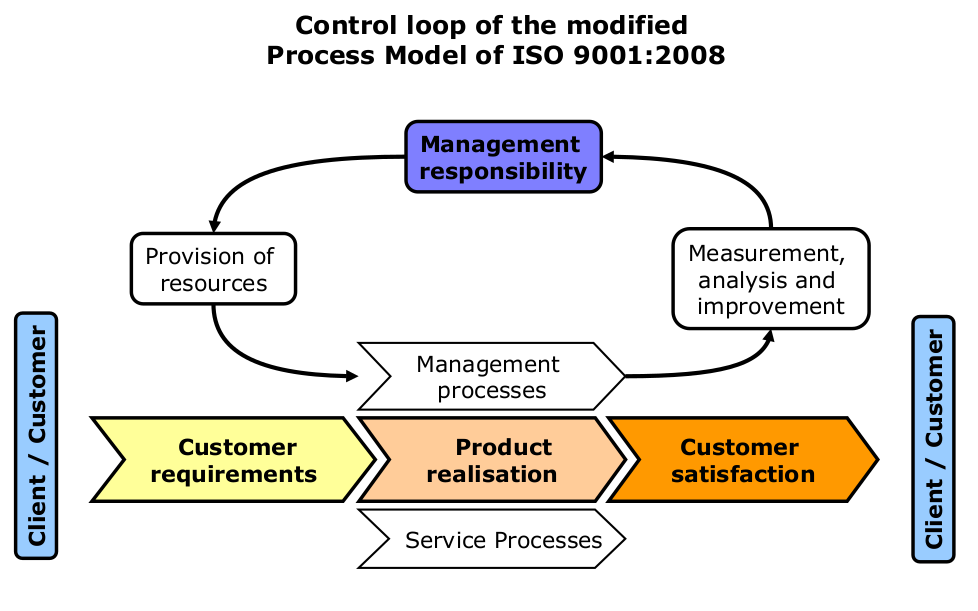
\includegraphics[width=\textwidth]{2.png}
\end{center}
\end{frame}

\begin{frame}{ISO 9000}
ISO 9000 is a set of general quality assurance standards to \textbf{assess}
the process quality of enterprises. It is a descriptive standard and not
directed towards improvement of process quality (although can be used for such
an improvement in combination with other tools).
\end{frame}

\begin{frame}{Models and Metamodels}
\begin{center}
  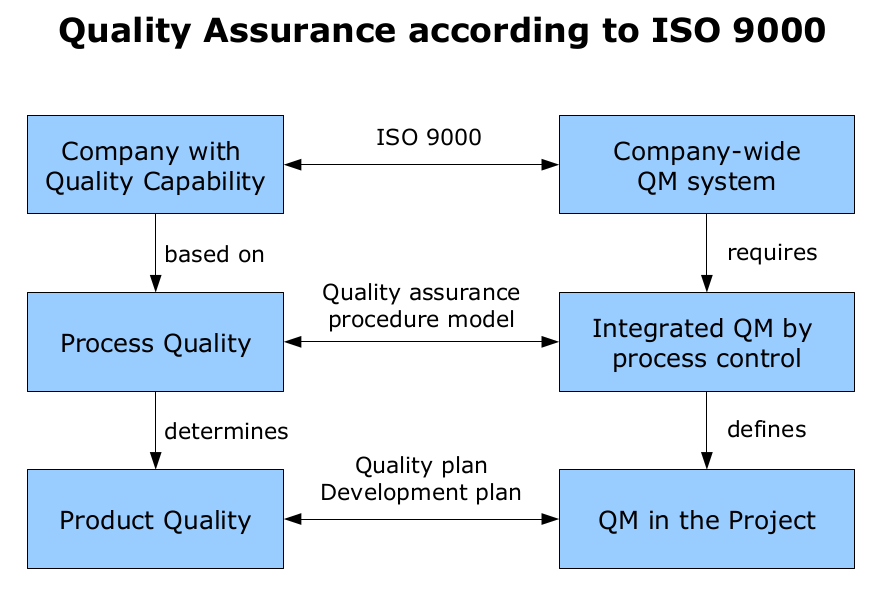
\includegraphics[width=\textwidth]{1.png}
\end{center}
\end{frame}

\begin{frame}{Managing Organisational Development}
Management is only possible in the context of a clear understanding of the
structural and procedural organisation of the organisation.  In order to
capture this in descriptive terms, a \textbf{separation of functions and
  resources} is necessary. In particular, "human resources" are removed from
the description and replaced by the term \textbf{role}.

In this way, a \emph{functional decoupling from the resources} is achieved at
design time -- only at runtime this position must be connected "just in time"
with a qualified resource that was produced beyond the horizon of the concrete
planning processes.
\end{frame}
\begin{frame}{Managing Organisational Development}
Only with such a decoupling (and only at the level of such a decoupling) it is
possible as management to take an external standpoint on its own activities.
Only in this way is \textbf{structurally driven organisational development}
possible. There are other culturally driven approaches such as TQM, which will
be discussed separately (the Toyota model).

Systematic management through structurally driven organisational development
means above all the creation and improvement of conditions for the management
of well-structured processes.
\end{frame}

\begin{frame}{Managing Organisational Development based on CMMI}
\begin{center}
  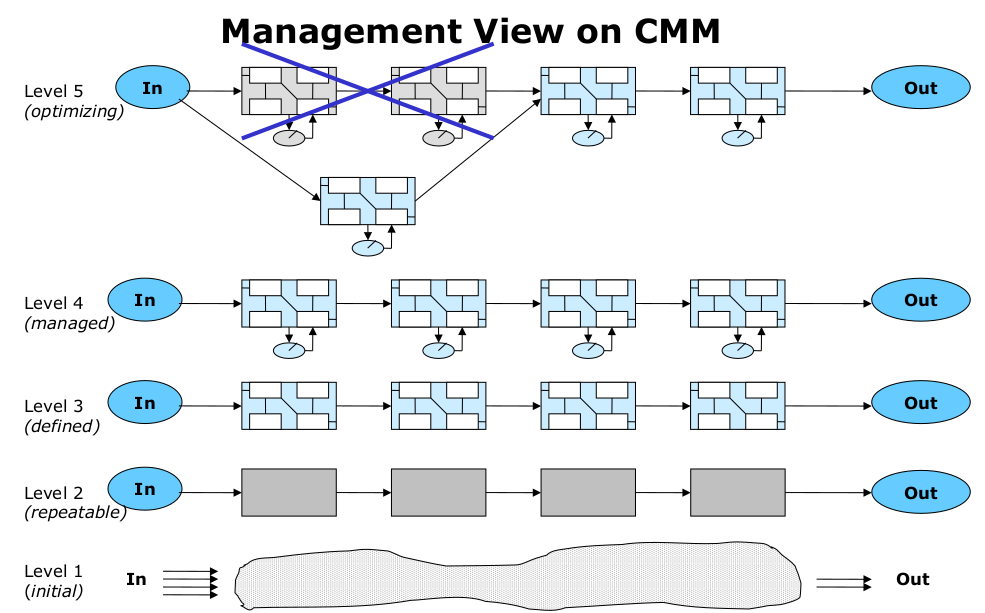
\includegraphics[width=\textwidth]{6.png}\\[1em] Increasing
  maturity of structured project management\\ within CMM(I)
\end{center}
\end{frame}
\end{document}
